%% ----------------------------------------------------------------
%% OverallApproach.tex
%% ----------------------------------------------------------------
\chapter{Overall Approach}
\label{Chapter:Overall Approach}

\begin{preamble}
	To create a high quality framework an overall approach for the project was decided on.

	This was done by first summarising the research conducted into previous work, as well as defining where this project fits within that ecosystem. Specific requirements were gathered from the client and an analysis of the needs of other project stakeholders conducted. This led to a list of requirements that the project would need to meet. Additionally, thought was put into the general system design of the framework.
\end{preamble}

\section{Reviewing Previous Work}
\label{Section:Reviewing Previous Work}
Having reviewed the Previous Work (\autoref{Chapter:Previous Work}), some design decisions for the project could be proposed to the client:
\begin{itemize}
	\item A basic quiz standard would need to be defined to allow interoperability between the authoring tool and questions overlay. It was decided not to use the \gls{QTI} standard to define the question sets due to the complexity of the standard, and the difficulty of implementing accessibility. The time constraint on this project would mean that more time would be spent on ensuring compliance with \gls{QTI} than implementing the tools.

	\item The interactive video had to be able to provide immediate feedback, to allow effective formative assessment to take place.

	\item A \gls{HTML5} video player would be used to play the videos, enabling mobile devices that do not support Flash to play the interactive videos. Using \gls{HTML5} for the control elements would also simplify the implementation of keyboard accessibility.

	\item The questions overlay would need to emit events that can be captured and used to analyse the users' viewing patterns. This would allow viewing patterns to be compared and contrasted with traditional videos.
\end{itemize}

\section{Client Requirements}
Because the long-term aim is to integrate this project into the new version of Synote, there were some specific requirements that our client had with regards to implementation.

The new version of Synote will be written in \gls{AngularJS} and \gls{HTML5}. To make it more easily compatible the questions overlay should also be written using this framework. With this new requirement it was agreed that \gls{Videogular}\footnote{\url{https://github.com/2fdevs/videogular}}\footnote{\url{https://github.com/2fdevs/bower-videogular-controls}} should be used. \gls{Videogular} is a \gls{HTML5} video player for \gls{AngularJS}. The nature of the library makes it very easy to write plugins to add the required functionality.

In addition to quizzes, the inclusion of polls must be supported within the questions overlay.

\subsection{AngularJS}
\label{Section:AngularJS}

\gls{AngularJS}\footnote{\url{https://angularjs.org/}} is a JavaScript Framework that extends HTML attributes. It is an open source library made by Google.

The underlying architectural pattern used by \gls{AngularJS} is client side \gls{MVC}. This is where the data (Model), appearance (View) and actions that can be applied (Controller) are separated out to make encapsulation and code reuse easier.

The framework allows custom HTML tags and attributes to be created using directives. Directives allow the user to specify the behaviour of specific elements they have created.

One of \gls{AngularJS}'s most prominent features is its use of two-way data binding. This synchronises the views with the data held in the model. This is especially useful when dealing with dynamic content, as when extra content is added it is automatically shown in the view.

\section{Stakeholder Analysis}
To decide on an approach for the project the stakeholders needed to be identified and analysed. Their requests have been prioritised by categorising each stakeholder (see \autoref{fig:Stakeholder matrix}).

\begin{figure}[h!]
	\centering
	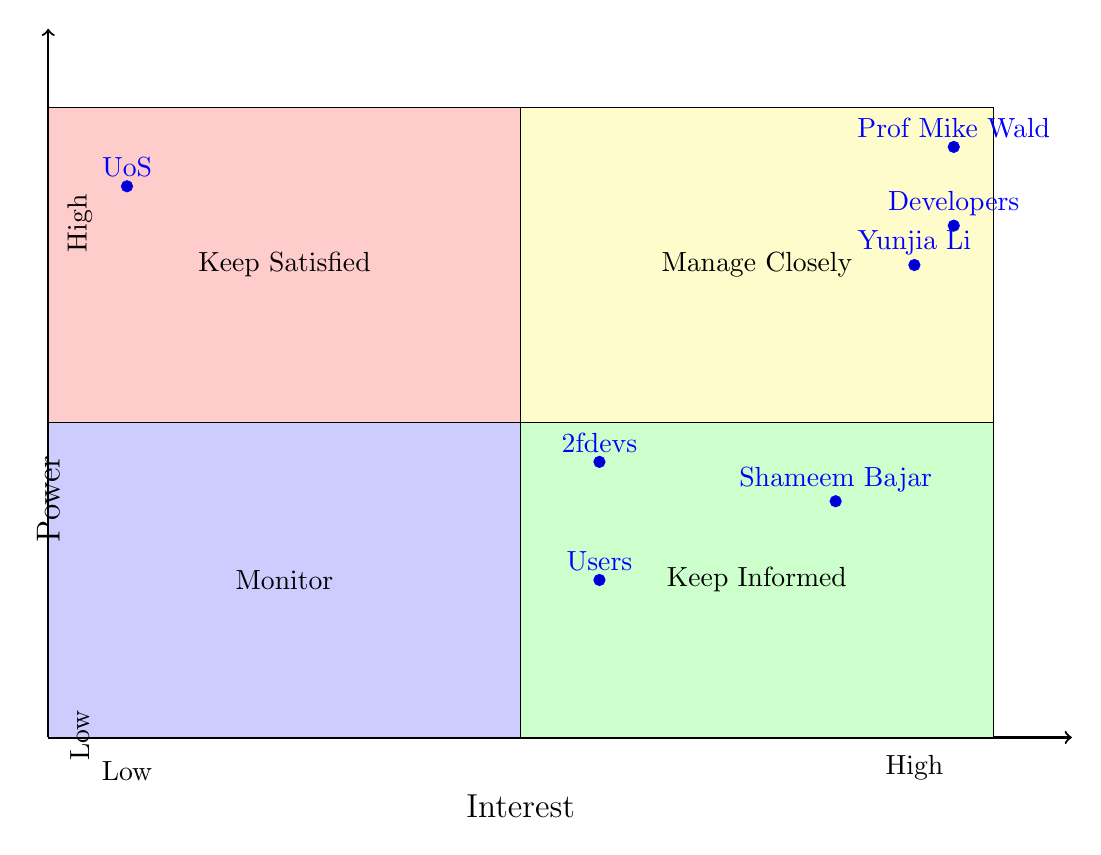
\begin{tikzpicture}[font=\rmfamily]
\draw [thick,->]  (0,0) -- coordinate (x axis mid) (13,0);
\draw [thick,->]  (0,0) -- coordinate (y axis mid) (0,9);
\filldraw[fill=blue!20!white, draw=black] (0,0) rectangle (6,4) node[pos=.5] {Monitor};
\filldraw[fill=green!20!white, draw=black] (6,0) rectangle (12,4) node[pos=.5] {Keep Informed};
\filldraw[fill=red!20!white, draw=black] (0,4) rectangle (6,8) node[pos=.5] {Keep Satisfied};
\filldraw[fill=yellow!20!white, draw=black] (6,4) rectangle (12,8) node[pos=.5] {Manage Closely};
%labels      
\node[xshift=-0.5cm, below=0.6cm] (xlabel) at (x axis mid) {{\large Interest}};
\node[rotate=90, left=0.8cm] (ylabel) at (y axis mid) {{\large Power}};
\begin{axis}[nodes near coords, xmin=0, xmax=13, ymin=0, ymax=9, width=13cm, height=9cm, axis x line=none, axis y line=none, scale only axis, enlargelimits=false]
\addplot+[only marks, point meta=explicit symbolic] coordinates { 
(11.5,7.5) [Prof Mike Wald] 
(7,3.5) [2fdevs] 
(10,3) [Shameem Bajar] 
(11,6) [Yunjia Li] 
(11.5,6.5) [Developers] 
(7, 2) [Users]
(1,7) [UoS]
 };
\end{axis}
\node[xshift=-5cm, above=0.2cm] at (xlabel) {Low};
\node[xshift=5cm, above=0.2cm] at (xlabel) {High};
\node[xshift=0.4cm,yshift=-3cm, rotate=90] at (ylabel) {Low};
\node[xshift=0.4cm,yshift=3.5cm, rotate=90] at (ylabel) {High};
\end{tikzpicture}
	\caption{Stakeholder matrix for the project\label{fig:Stakeholder matrix}}
\end{figure}

Our supervisor and client, Professor Mike Wald, had the most interest and power in the project. As the project proposer it would be his ideas that would form the basis of the project.

Yunjia Li is the lead developer for the new version of Synote. As the aim of the project was to provide code for Synote he had a lot of interest in the project. His requirements would need to be taken into account to ensure interoperability between the two systems, which gave him power in the project.

Due to the nature of the project the developers themselves would be major stakeholders. Work would need to be evenly distributed to give all members of the group the same opportunities to obtain marks.

The University of Southampton sets the mark scheme and guidelines for the project. These would need to be satisfied to make the project successful.

2fdevs are the development team who created the \gls{Videogular} player. The project would be creating plugins for this player, and so would rely on certain attributes of \gls{Videogular}, such as accessibility.

Shameem Bajar is a 3rd year student who has an Individual Project based around this project. Her interest levels would be high as her work depends on the output of this project.

The users would be stakeholders, as the decisions made will affect how easy the system is to use and whether the desired functionality is available.

Requirements from all stakeholders will be considered but any conflicts will be dealt with by prioritising the needs of the most influential party (closer to the top right of \autoref{fig:Stakeholder matrix}).

\section{Requirements Analysis}
\label{Section:Requirements Analysis}
Considering the needs of all stakeholders, a set of requirements for the project were agreed. The reasons for each being included are specified in italics.

\subsection{Functional Requirements}
\begin{requirement}[label=\textbf{F\arabic*}]
	\item \textbf{Question types}  \label{Req:Question types} \hfill \\ 
		The questions overlay must be able to display multiple choice (with one or more selectable answers), range selector, rating, and text based answer types. The stakeholders for each are described in italics after each one.

		\textit{Authors wish to ask questions that require set responses.}

	\item \textbf{Jumping to content} \label{Req:Jumping to content} \hfill \\ 
		There should be a feature to jump to specific content if a question is answered incorrectly.

		\textit{This is a method of giving instant feedback, which was one of the things found to be important in the Previous Work (see \autoref{Chapter:Previous Work}).}

	\item \textbf{Analytics events} \label{Req:Analytics events} \hfill \\ 
		Video and question events should be emitted from the questions overlay so that analytics data can be calculated.

		\textit{Analysis of existing work showed a lack of analysis of video usage behaviour, so this would help facilitate new analysis.}

	\item \textbf{Cuepoints} \label{Req:Cuepoints} \hfill \\ 
		The locations of the questions should be marked visually on the \gls{scrub bar} of the video.

		\textit{Users wish to see where the questions are in the video.}

	\item \textbf{Poll responses} \label{Req:Poll responses} \hfill \\ 
		The responses to polls must be able to be sent to a server, and results from the server must be able to be displayed.

		\textit{This is one of our client's requirements.}

	\item \textbf{Instant feedback} \label{Req:Instant feedback} \hfill \\ 
		Once a question or set of questions have been answered there must be a way of receiving instant feedback on performance.

		\textit{Found to be important in the analysis of existing work.}
\end{requirement}

\subsection{Non-Functional Requirements}
\begin{requirement}[label=\textbf{N\arabic*}]
	\item \textbf{Video player used} \label{Req:Video player used} \hfill \\ 
		\gls{Videogular} should be used as the video player, and components should be written in \gls{AngularJS} and \gls{HTML5}.

		\textit{One of Yunjia's requirements.}

	\item \textbf{Standalone} \label{Req:Standalone} \hfill \\ 
		The plugins created should be standalone, but still easy to integrate into the new version of Synote.

		\textit{One of the client's requirements.}

	\item \textbf{Browser compatibility} \label{Req:Browser compatibility} \hfill \\ 
		The questions overlay must work on Microsoft Internet Explorer 8, Mozilla Firefox and Google Chrome.

		\textit{One of the client's requirements.}

	\item \textbf{Operating System Compatibility} \label{Req:OS compatibility} \hfill \\ 
		The questions overlay must work on Windows, Mac OS X and Android.

		\textit{One of the client's requirements.}

	\item \textbf{Extensibility} \label{Req:Extensibility} \hfill \\ 
		The questions overlay must be extensible so that further features can be added. 

		\textit{Makes incremental development easier for the developers, and allows any missing features that are wanted for integration into Synote to be added easily.}

	\item \textbf{Keyboard Accessibility}\label{Req:Keyboard accessibility} \hfill \\ 
		The questions overlay and authoring tool must be completely accessible to a keyboard-only user.

		\textit{Users may not be able to use a mouse.}

	\item \textbf{Use of colour}\label{Req:Use of colour} \hfill \\ 
		Any colours used should be customisable.

		\textit{Users may have visual impairments such as colour blindness, so they may only be able to use the application if it is in certain colours.}

	\item \textbf{User interface} \label{Req:User interface} \hfill \\ 
		A Graphical User Interface (GUI) must be provided for the Authoring Tool so that non-technical users can create quizzes.

		\textit{One of the client's requirements is to reduce the barrier to entry.}

	\item \textbf{User friendliness} \label{Req:User friendliness} \hfill \\ 
		To allow maximum use of these tools, no tools should not require extensive training.

		\textit{One of the client's requirements is to reduce the barrier to entry.}

	\item \textbf{Documentation and Testing Examples} \label{Req:Documentation} \hfill \\ 
		The plugins built should have usage examples, to allow less technical users to implement their own system.

		\textit{One of the client's requirements is to reduce the barrier to entry, and to ensure that the framework is easy to integrate.}

	\item \textbf{Server architecture} \label{Req:Server architecture} \hfill \\ 
		Any server behaviour should be accessed by \gls{REST} calls, which should work across hosts.

		\textit{One of Yunjia's requirements to allow easier integration into Synote.}

	\item \textbf{Scalability} \label{Req:Scalability} \hfill \\ 
		All tools should scale when they are used by large numbers of people.

		\textit{One of the client's requirements is to ensure performance does not degrade when use of the tools are scaled.}
\end{requirement}

\section{Modular Web server Approach}
\label{Section:Modular Approach}

It is important for our project to be easily integrated into other projects, particularly the latest version of Synote (see \autoref{Section:Synote}). To accomplish this the design of the back-end systems ensures that they can be run without depending on any other modules. All of the functionality will be accessible via \gls{REST} calls as set out by \cref{Req:Server architecture}.

Abstracting all calls using \gls{REST} means that other services are able to interact with the back-end services in a language independent way, which also makes the application standalone (\cref{Req:Standalone}). To facilitate this, all \gls{REST} responses are returned with a Cross-Origin header. This allows servers which are not on the same machine to communicate with the \gls{REST} service.

These features allow an external application to run the Web server separately and communicate with our server side code. The only dependency added by those who use the code in this project is that they need to be able to make \gls{REST} calls.

\section{System Architecture}

The following set of components were decided on, the interactions of which are shown in \autoref{fig:System architecture diagram}:

\begin{itemize}
	\item
		\textbf{Videogular Questions} displays questions over a \gls{Videogular} video player according to a quiz defined in a \gls{DF}. If any of the questions are polls, it sends responses of the poll(s) to a results server, and displays the results that are sent back.
	\item
		\textbf{Videogular Analytics} logs events from \gls{Videogular} (e.g. when the user plays or pauses the video) and Videogular Questions (e.g. when the user answers a question) and sends them to an analytics server.
	\item
		\textbf{Videogular Cuepoints} displays marks on the \gls{scrub bar} indicating when questions will appear.
	\item
		The \textbf{results server} receives responses from Videogular Questions and returns the aggregated results on request.
	\item
		The \textbf{analytics server} receives event logs from Videogular Analytics, and provides a separate Web front-end, the \textbf{analytics front-end}, which displays analysis of the events.
	\item
		\textbf{Videogular Heatmap} overlays a heat map onto the \gls{scrub bar} of the \gls{Videogular} player, for visualisation of analytics results.
	\item
		An \textbf{authoring tool} allows a user to create \glspl{DF} without having to write them manually.
\end{itemize}

\begin{figure}[h!]
	\centering
	\begin{tikzpicture}[
  font=\sffamily,
  every matrix/.style={ampersand replacement=\&,column sep=2cm,row sep=2cm},
  source/.style={draw,thick,rounded corners,fill=yellow!20,inner sep=.3cm},
  vg-plugin/.style={draw,thick,rounded corners,fill=yellow!20,inner sep=.3cm},
  videogular/.style={draw,thick,circle,fill=blue!20},
  process/.style={draw,thick,circle,fill=blue!20},
  sink/.style={source,fill=green!20},
  datastore/.style={draw,very thick,shape=datastore,inner sep=.3cm},
  server/.style={source,fill=green!20},
  dots/.style={gray,scale=2},
  to/.style={->,>=stealth',shorten >=1pt,semithick,font=\sffamily\footnotesize},
  between/.style={<->,>=stealth',shorten >=1pt,semithick,font=\sffamily\footnotesize},
  every node/.style={align=center}]

  % Position the nodes using a matrix layout
  \matrix{
    \node[vg-plugin] (cuepoints) {cuepoints};
      \&
      \& \node[vg-plugin] (questions) {questions};
      \& \node[server] (poll-server) {poll server}; \\

    \& \node[videogular] (videogular) {videogular}; \\

    \node[vg-plugin] (heatmap) {heatmap};
      \&
      \& \node[vg-plugin] (analytics) {analytics};
      \& \node[server] (analytics-server) {analytics server}; \\
  };

  \draw[between] (questions) --
      node[midway,above] {user responses}
      node[midway,below] {results} (poll-server);
  \draw[to] (questions) --
      node[midway,right] {user interactions}
      (analytics);
  \draw[to] (questions) --
      node[midway,above] {question times}
      (cuepoints);
  \draw[between] (analytics) --
      node[midway,above] {data}
      node[midway,below] {acks} (analytics-server);
  \draw[to] (analytics-server) to[bend left=15] node[midway,above] {events}
      node[midway,below] {level 1} (heatmap);
  \draw[between] (videogular) -- (cuepoints);
  \draw[between] (videogular) -- (analytics);
  \draw[between] (videogular) -- (questions);
  \draw[between] (videogular) -- (heatmap);
\end{tikzpicture}

	\caption{System architecture diagram for the project \label{fig:System architecture diagram}}
\end{figure}

The results and analytics servers (including the analytics front-end) are examples only, and not themselves deliverables (see \autoref{Section:Deliverables}).

As the expected behaviour of our plugins depends on the application they are used in, an example site was required to test the other components.

The server components were separated as they do completely separate jobs, and because some deployments may use one but not the other. Similarly, Videogular Analytics is separate from Videogular Questions as it only depends on \gls{Videogular}. Videogular Cuepoints and Videogular Heatmap are separate components as they can be used in other, completely unrelated projects.

\newpage %only the first line was on the page
\section{Deliverables}
\label{Section:Deliverables}

The following set of deliverables was agreed on in order to meet the requirements:

\begin{itemize}
	\item Videogular Questions: a plugin for adding polls and questions to videos
		\begin{itemize}
			\item Source code, under the MIT licence
			\item An example proof-of-concept website
		\end{itemize}
	\item Videogular Cuepoints: a plugin which displays informational marks on the \gls{scrub bar} of a video
		\begin{itemize}
			\item Source code, under the MIT licence
			\item Demonstration of usage in Videogular Questions example site
		\end{itemize}
	\item Videogular Analytics: a plugin for reporting of events within the Videogular player
		\begin{itemize}
			\item Source code, under the MIT licence
			\item An API specification for Videogular Analytics
			\item An example site showing basic usage of the analytics data collected by the plugin
		\end{itemize}
	\item Videogular Heatmap: a plugin which displays heat map information on the \gls{scrub bar} of a video
		\begin{itemize}
			\item Source code, under the MIT licence
			\item Demonstration of usage in Videogular Analytics example site
		\end{itemize}
	\item Authoring tool: a Web application to produce the \gls{DF} to be used with Videogular Questions
		\begin{itemize}
			\item Source code, under the MIT licence
		\end{itemize}
\end{itemize}


\section{Testing}
\label{Section:Overall_Testing}

Software testing is necessary on projects of all sizes, especially on large projects such as this. To ensure quality throughout the project each part of the framework has been thoroughly tested.

In this project, this was done by creating example sites, satisfying \cref{Req:Documentation}. Due to the free-form nature of AngularJS's project structure one of the industry standards, angular-seed\footnote{\url{https://github.com/angular/angular-seed}}, was used. angular-seed is a skeleton with which one can create AngularJS Web apps. It includes two testing frameworks (Karma and Jasmine) already set up. More details about Karma, Jasmine and other tests performed can be found in \autoref{Chapter: Testing}.

